% Options for packages loaded elsewhere
\PassOptionsToPackage{unicode}{hyperref}
\PassOptionsToPackage{hyphens}{url}
%
\documentclass[
]{article}
\usepackage{amsmath,amssymb}
\usepackage{lmodern}
\usepackage{iftex}
\ifPDFTeX
  \usepackage[T1]{fontenc}
  \usepackage[utf8]{inputenc}
  \usepackage{textcomp} % provide euro and other symbols
\else % if luatex or xetex
  \usepackage{unicode-math}
  \defaultfontfeatures{Scale=MatchLowercase}
  \defaultfontfeatures[\rmfamily]{Ligatures=TeX,Scale=1}
\fi
% Use upquote if available, for straight quotes in verbatim environments
\IfFileExists{upquote.sty}{\usepackage{upquote}}{}
\IfFileExists{microtype.sty}{% use microtype if available
  \usepackage[]{microtype}
  \UseMicrotypeSet[protrusion]{basicmath} % disable protrusion for tt fonts
}{}
\makeatletter
\@ifundefined{KOMAClassName}{% if non-KOMA class
  \IfFileExists{parskip.sty}{%
    \usepackage{parskip}
  }{% else
    \setlength{\parindent}{0pt}
    \setlength{\parskip}{6pt plus 2pt minus 1pt}}
}{% if KOMA class
  \KOMAoptions{parskip=half}}
\makeatother
\usepackage{xcolor}
\usepackage[margin=1in]{geometry}
\usepackage{graphicx}
\makeatletter
\def\maxwidth{\ifdim\Gin@nat@width>\linewidth\linewidth\else\Gin@nat@width\fi}
\def\maxheight{\ifdim\Gin@nat@height>\textheight\textheight\else\Gin@nat@height\fi}
\makeatother
% Scale images if necessary, so that they will not overflow the page
% margins by default, and it is still possible to overwrite the defaults
% using explicit options in \includegraphics[width, height, ...]{}
\setkeys{Gin}{width=\maxwidth,height=\maxheight,keepaspectratio}
% Set default figure placement to htbp
\makeatletter
\def\fps@figure{htbp}
\makeatother
\setlength{\emergencystretch}{3em} % prevent overfull lines
\providecommand{\tightlist}{%
  \setlength{\itemsep}{0pt}\setlength{\parskip}{0pt}}
\setcounter{secnumdepth}{-\maxdimen} % remove section numbering
\ifLuaTeX
  \usepackage{selnolig}  % disable illegal ligatures
\fi
\IfFileExists{bookmark.sty}{\usepackage{bookmark}}{\usepackage{hyperref}}
\IfFileExists{xurl.sty}{\usepackage{xurl}}{} % add URL line breaks if available
\urlstyle{same} % disable monospaced font for URLs
\hypersetup{
  pdftitle={eMOLT Update},
  pdfauthor={George Maynard},
  hidelinks,
  pdfcreator={LaTeX via pandoc}}

\title{eMOLT Update}
\author{George Maynard}
\date{2024-10-18}

\begin{document}
\maketitle

\emph{eMOLT Update 2024-10-18 }

\hypertarget{weekly-recap}{%
\subsection{Weekly Recap}\label{weekly-recap}}

Despite the shortened week, it's been a productive one for the eMOLT
team. First off, a big thanks to Huanxin for dropping everything to run
up to the F/V Gladys Elaine in New Hampshire on Wednesday. The deckbox
wasn't connecting to the Gulf of Maine Lobster Foundation's remote
support system and the vessel was scheduled to leave for a trip on
Wednesday around noon, so Huanxin drove up and got everything running
again. Thanks to Erin and Captain Pete for coordinating all of that.

Thanks also to everyone up in Maine for your communication and patience
as we work through upgrading the last few deckboxes that still have the
old software and iron out kinks with the new Lowell TD loggers. Captain
Curt on the F/V Lil' More Tail, Captain Sherm on the F/V Freedom,
Captain Joe Sr.~on the F/V Joseph and Peter, Captain Joey Jr.~on the F/V
Jasmine Marie, and Dr.~Goode from the University of Maine have all been
in touch this week to make sure their systems are up and running. We
really appreciate your efforts!

Finally, thanks to Captain Peter, his crew, and the team from
Coonamessett Farm Foundation for your work yesterday rigging up an eMOLT
system aboard the F/V Atlantic. The deckbox install was less complicated
than we feared, but we definitely all learned some valuable lessons
figuring out how to install the sensor and housing. Captain Peter's
welding gave us a few mounting options we wouldn't have had otherwise.
This is the CFF team's first install, and we look forward to partnering
with them on many more!

\begin{figure}
\centering
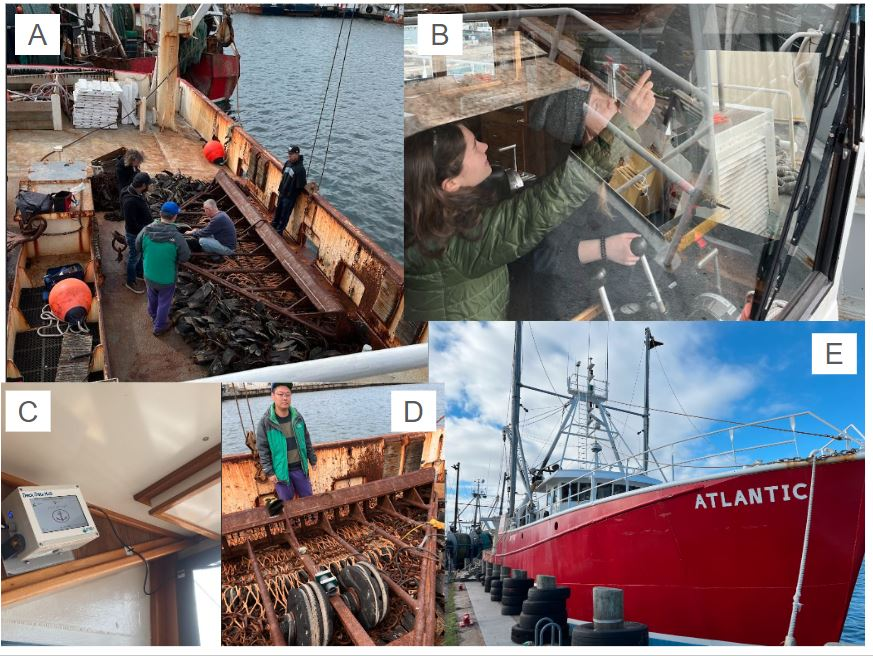
\includegraphics{Atlantic_collage.JPG}
\caption{collage of images from F/V Atlantic installation}
\end{figure}

\begin{quote}
\emph{Figure 1 -- Installation of an eMOLT system aboard the F/V
Atlantic. A) Farrell, Samir, and Huanxin consult with the captain and
crew about sensor placement. B) Cassie and Tori installing the deckbox
and bluetooth extension antenna in the wheelhouse. C) The finished
deckbox install. D) Huanxin with the newly installed sensor. E) The F/V
Atlantic tied up in New Bedford.}
\end{quote}

This week, the eMOLT fleet recorded 103 tows of sensorized fishing gear
totaling 1800 sensor hours underwater. The warmest recorded bottom
temperature was 65.6 F south of Fire Island in approximately 20 fathoms
(red profile) and the coldest recorded bottom temperature was 44.5 F out
by the Hague Line on southeast Georges in approximately 121 fathoms
(blue profile). Below, you can see these profiles plus a few other
temperature profiles of interest across the region from the last week.

Seasonal stratification is still evident on Stellwagen Bank (pink) and
off the New Hampshire Seacoast (yellow), but is breaking down along the
Maine coast (purple and aqua).

\begin{figure}
\centering
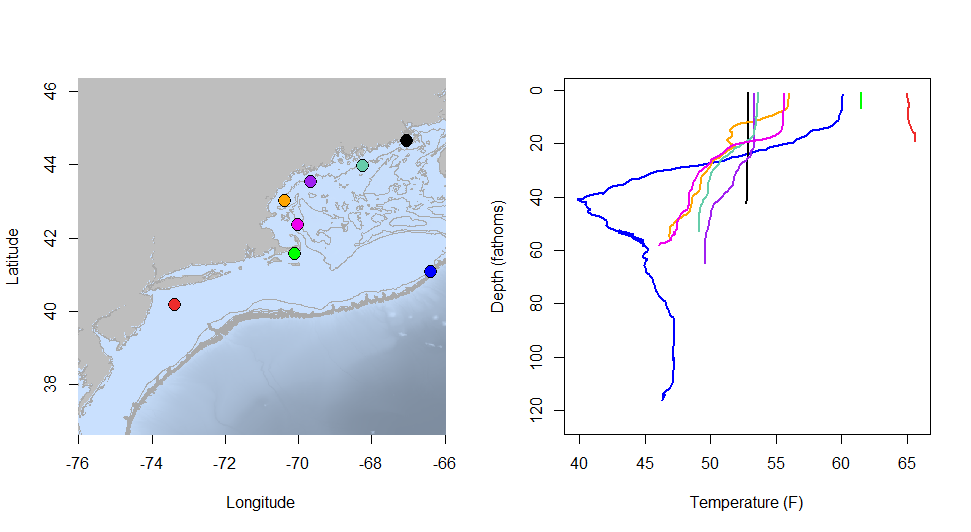
\includegraphics{profiles.png}
\caption{profiles from this week}
\end{figure}

\begin{quote}
\emph{Figure 2 -- Temperature profiles collected by eMOLT participants
over the last week. The blue profile is where the coldest bottom
temperature was measured and the red profile is where the warmest bottom
temperature was measured. All other colors are assigned randomly.
Colored points on the map indicate where profiles of the same color were
collected.}
\end{quote}

\hypertarget{northeast-cooperative-research-summit-registration-waitlist-open}{%
\subsection{Northeast Cooperative Research Summit Registration Waitlist
Open}\label{northeast-cooperative-research-summit-registration-waitlist-open}}

We are at capacity for the 2025 Northeast Cooperative Research Summit.
Any new registrants will be added to the waitlist for this event.

We have officially booked
\href{https://maps.app.goo.gl/TRsvzYP6AogdDMXW9}{The Westin Portland
Harborview} for the 2025 Northeast Cooperative Research Summit, which
will be held on January 28th, 2025! Please mark your calendars. The web
pages are live and information about registering and presenting at the
summit is available
\href{https://www.fisheries.noaa.gov/event/2025-northeast-cooperative-research-summit}{here}.
Please reach out to
\href{https://www.fisheries.noaa.gov/contact/thomas-swiader}{Thomas
Swiader} with any questions. Registration closes on November 8, 2024.
This year, in addition to the Summit itself, we're working with partners
offer tours of some facilities down on the waterfront in Portland the
day before. Currently, the plan is to visit the Portland Fish Exchange,
Ready Seafood, and the Gulf of Maine Research Institute. We'll have more
information about how to register for the tours in the coming weeks.

\hypertarget{system-hardware-upgrade-list}{%
\subsubsection{System Hardware Upgrade
List}\label{system-hardware-upgrade-list}}

The following vessels remain on our list for hardware upgrades. If you
aren't on the list and think you should be, please reach out. \emph{Note
that this list is different from our new install queue.}

\begin{quote}
\begin{itemize}
\tightlist
\item
  F/V Brooke C *
\item
  F/V Excalibur
\item
  F/V Kaitlyn Victoria
\item
  F/V Kyler C
\item
  F/V Linda Marie
\item
  F/V Nathaniel Lee *
\item
  F/V Noella C
\item
  F/V Sao Paulo
\item
  F/V Sea Watcher I
\item
  F/V Virginia Marise
\end{itemize}
\end{quote}

\hypertarget{dissolved-oxygen-in-cape-cod-bay}{%
\subsubsection{\texorpdfstring{\href{https://experience.arcgis.com/experience/0d553dfc6c60487cb1f4d20b5366ee0b/page/Map-Page/}{Dissolved
Oxygen in Cape Cod
Bay}}{Dissolved Oxygen in Cape Cod Bay}}\label{dissolved-oxygen-in-cape-cod-bay}}

\hypertarget{courtesy-of-the-massachusetts-division-of-marine-fisheries-and-the-massachusetts-lobstermens-association}{%
\paragraph{Courtesy of the Massachusetts Division of Marine Fisheries
and the Massachusetts Lobstermen's
Association}\label{courtesy-of-the-massachusetts-division-of-marine-fisheries-and-the-massachusetts-lobstermens-association}}

The ``very low'' oxygen conditions shown here in orange are mostly from
earlier this week. More recent readings from the later half of the week
are ``low'' (yellow) or ``normal'' (green).

\begin{figure}
\centering
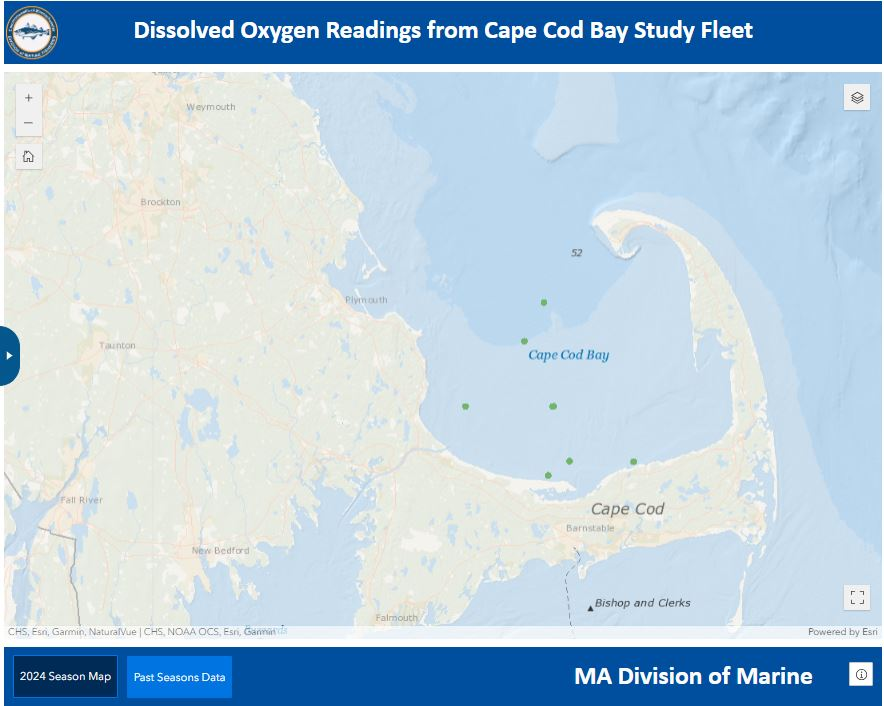
\includegraphics{CCB_screenshot.JPG}
\caption{CCB Screenshot}
\end{figure}

\begin{quote}
\emph{Figure 3 -- Dissolved oxygen observations from Cape Cod Bay
collected by participants in the eMOLT program and the Cape Cod Bay
Study Fleet program operated by Massachusetts Division of Marine
Fisheries and the Massachusetts Lobstermen's Association over tthe past
week. Green dots indicate dissolved oxygen values in the normal range
(\textgreater{} 6 mg/L), yellow dots indicate low dissolved oxygen
values (4-6 mg/L), orange dots indicate very low dissolved oxygen values
(2-4 mg/L), and red dots indicate critically low values (\textless{} 2
mg/L).}
\end{quote}

\hypertarget{bottom-temperature-forecasts}{%
\subsubsection{Bottom Temperature
Forecasts}\label{bottom-temperature-forecasts}}

\hypertarget{doppio}{%
\paragraph{Doppio}\label{doppio}}

This week, \textasciitilde49\% of bottom temperature observations were
within 2 degrees (F) of the Doppio forecasted value at those points. The
bottom temperature forecast performed best around Cape Cod. Observed
temperatures were warmer than expected east of New Jersey, along the
Maine Coast, and on southeastern Georges Bank.

\begin{figure}
\centering
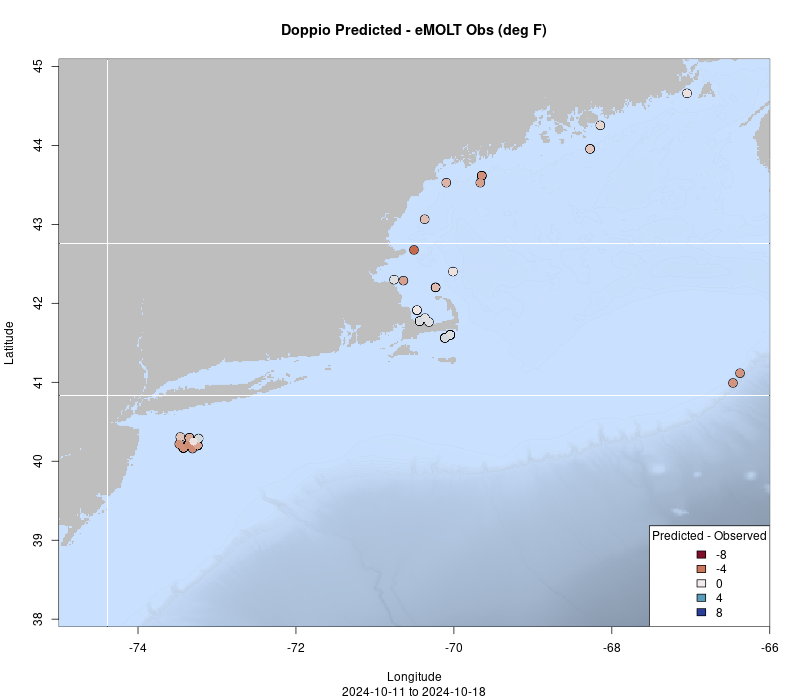
\includegraphics{doppio_compare.png}
\caption{Doppio performance}
\end{figure}

\begin{quote}
\emph{Figure 4 -- Performance of the Doppio forecast's bottom
temperature layer over the last week relative to observations collected
by eMOLT participants. Red dots indicate areas where bottom temperature
observations were warmer that predicted. Blue dots indicate areas where
bottom temperature observations were cooler than predicted. Bottom
temperature observations are compared with the most recent forecast run
available before the observation was made.}
\end{quote}

\begin{figure}
\centering
\includegraphics{DOPPIO_forecast_F.gif}
\caption{Doppio Forecast}
\end{figure}

\begin{quote}
\emph{Figure 5 -- The most recent Doppio bottom temperature forecast.
The gray line is the 50 fathom line and the black line is the hundred
fathom line. Purple shades indicate cooler water.}
\end{quote}

\hypertarget{northeast-coastal-ocean-forecast-system}{%
\paragraph{Northeast Coastal Ocean Forecast
System}\label{northeast-coastal-ocean-forecast-system}}

\begin{figure}
\centering
\includegraphics{NECOFS_GOM.gif}
\caption{NECOFS plot}
\end{figure}

\begin{quote}
\emph{Figure 6 -- The most recent bottom temperature forecast from the
Northeast Coastal Ocean Forecast System GOM7 model. Purple shades
indicate cooler water.}
\end{quote}

\begin{figure}
\centering
\includegraphics{NECOFS_MABAY.gif}
\caption{Mass Bay plot}
\end{figure}

\begin{quote}
\emph{Figure 7 -- The most recent bottom temperature forecast from the
Northeast Coastal Ocean Forecast System MassBay model. Purple shades
indicate cooler water.}
\end{quote}

\hypertarget{bycatch-reduction-engineering-program-pre-proposals-due-dec.-13}{%
\subsection{Bycatch Reduction Engineering Program Pre-Proposals Due
Dec.~13}\label{bycatch-reduction-engineering-program-pre-proposals-due-dec.-13}}

The
\href{https://www.fisheries.noaa.gov/national/bycatch/bycatch-reduction-engineering-program}{Bycatch
Reduction Engineering Program} provides funding to support applied
management projects and activities to reduce bycatch. Bycatch reduction
is a top priority for NOAA Fisheries, as outlined in our
\href{https://www.fisheries.noaa.gov/national/bycatch/national-bycatch-reduction-strategy}{National
Bycatch Reduction Strategy}.

For more information about program priorities and how to apply, please
visit the
\href{https://www.fisheries.noaa.gov/grant/bycatch-reduction-engineering-program-funding}{BREP
Funding Website}.

\hypertarget{cooperative-research-opportunity-free-airmar-weather-stations}{%
\subsection{Cooperative Research Opportunity -- FREE Airmar Weather
Stations}\label{cooperative-research-opportunity-free-airmar-weather-stations}}

Our partners at Ocean Data Network, based out of Portland, Maine are
looking for fishing vessels operating in the Gulf of Maine that are
interested in receiving a \textbf{FREE Airmar weather station}
installation this fall. The weather data stream will integrate with the
wheelhouse electronics to give captains real time weather data on their
navigation software while recording and sending the data to the National
Weather Service to improve offshore weather forecasting for everyone
operating in the region! In order to qualify, a vessel must have a NMEA
2000 vessel electronics system and relatively modern navigation
software, such as Time Zero, if they want to be able to visualize the
data in the wheelhouse. The system will provide air temperature,
barometric pressure, wind speed, and wind direction in real time. This
is a pilot project looking for ten vessels to participate. Vessels need
to fish close to year-round. If you're fishing hard, have these
electronics on board, and want to help improve offshore forecasting
accuracy, please reach out to:

Jack Carroll
\href{mailto:jack@oceandata.net}{\nolinkurl{jack@oceandata.net}}

All the best,

-George and JiM

\end{document}
